\newpage

\subsection*{\Large{Постановка задачи}}

Задача построения оптимальных трасс линейных объектов выглядит следующим образом. На определенной территории, которую представляет собой поверхность в трёхмерном пространстве $\breve{S}$, описывающая земной рельеф задано множество объектов $\check{P} \in \breve{S}$, являющиеся точками. Требуется связать множество объектов $\check{P}$ коммуникационной сетью, так чтобы затраты на строительство данной сети были минимальны.
\par
Обозначим за область расчетов $Q$ проекцию поверхности $\breve{S}$ на плоскость $xOy$. 
При проектировании  $\check{P}$ на $Q$, будет получено множество объектов \mbox{$P = \{(x_i, y_i) \in Q , i=\overline{1..n}\}$}. Помимо области проектирования и объектов также заданы множество областей \\ \mbox{$A = \{\{x_{j},y_{j}\}_{j=1}^{n_i} \in Q, i=\overline{1..m}\}$} и множество существующих линейных объектов \\ \mbox{$L = \{\{x_{j},y_{j}\}_{j=1}^{n_i} \in Q, i=\overline{1..k}\}$}. 
Основываясь на стоимостях строительства в областях $A$ и вдоль линейных объектов $L$ задана функция строительных затрат \\ \mbox{$f: \{Q \rightarrow \mathbb{R}, \forall(x, y) \in Q: f(x, y) \ge 0\}$}, обозначающая стоимость строительства в каждой конкретной точке плоскости $Q$.
\par
В результате работы программы должна быть построена сеть линейных объектов \\
$L_{res} = \{\{x_{j},y_{j}\}_{j=1}^{n_i} \in Q$ оптимальная по заданным параметрам.
\par
Для нахождения оптимальной сети будем использовать граф. 
Для построения графа сгенерируем набор точек $D  = \{(x_i, y_i) \in Q\}$, на основе которых методом триангуляции Делоне получим вычислительную сетку и добавим её в граф $\mathbb{G} = \{\mathbb{V}, \mathbb{E}\}$, так что $\mathbb{V} \subseteq D$. Определим веса ребер графа $e = \{u,v\} \subseteq \mathbb{E}$, как функцию $\rho: \mathbb{V} \times \mathbb{V} \rightarrow \mathbb{R}$, где \\ $\rho(u, v) = d(u, v) \cdot \frac{f(u) + f(v)}{2} $, где $d:  \mathbb{V} \times \mathbb{V} \rightarrow \mathbb{R}$ - расстояние между двумя точками, лежащими на поверхности Земли в  метрах. Также обозначим за $w: \mathbb{G} \rightarrow \mathbb{R}$, где $w$ - сумма длин всех ребёр графа $\mathbb{G}$.

Если $T \subseteq V$, то $G$ называется графом, соединяющим $T$. При этом такой подграф $ST \subseteq G$, соединяющий $T$, минимально возможного веса $w(ST)$ является деревом, которое называется минимальным деревом Штейнера на $T$.

Терминальными точками назовем множество точек  $T \subseteq V$, между которыми требуется построить дерево Штейнера.

Точками Штейнера называется множество точек $P \subseteq V(ST) / T$.

Точками разветвления назовем подмножество точек Штейнера $S \subseteq P$, которые были добавлены во время работы алгоритма, реализующие лучшее решение, чем построенное только на терминальных точках.

Остовное дерево графа состоит из минимального подмножества рёбер графа, таких, что из любой вершины графа можно попасть в любую другую вершину, двигаясь по этим рёбрам.

Минимальное остовное дерево (или минимальное покрывающее дерево) в связанном взвешенном неориентированном графе — это остовное дерево этого графа, имеющее минимальный возможный вес, где под весом дерева понимается сумма весов, входящих в него рёбер.

\subsection*{\Large{Идея алгоритма}}
В литературе, в основном, представлены алгоритмы поиска оптимальных, использующие Евклидову метрику, которая не применима в нашем случае в связи с непостоянным значением функции $f$ на области расчетов $Q$, а также наличием рельефа. Алгоритмы поиска оптимальной сети на графах, будут неэффективны по времени работы в нашем случае, так как мы можем использовать знания о предметной области и подобрать эвристику, улучшающую, как точность решения, так и скорость его нахождения.

\begin{figure}[H]
	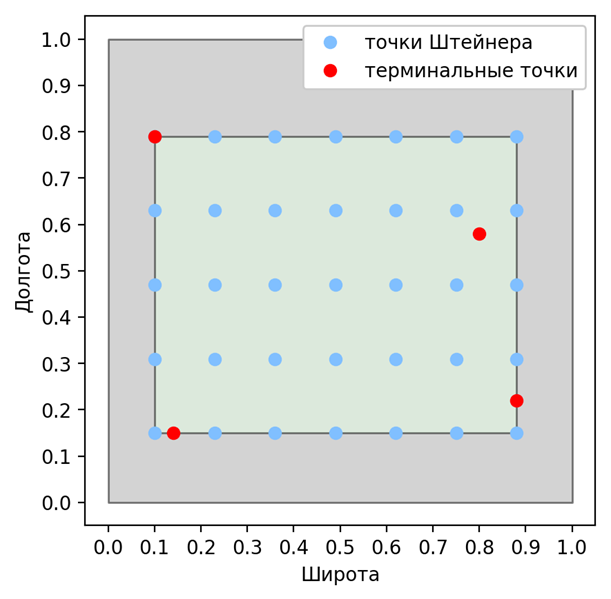
\includegraphics[width=0.7\textwidth]{images/4_1.png}
	\caption{Получение точек Штейнера}
\end{figure}
\vskip 4mm

Для начала, создается ограничительный прямоугольник, для которого мы генерируем набор точек разветвления. Мы разбиваем прямоугольник на $n_x$ точек по горизонтали и $n_y$ точек по вертикали. Итого, имеем $n_x \cdot n_y$  точек разветвления на плоскости (см. рис. 1). Для каждой точки разветвления мы находим ближайшую к ней по расстоянию вершину в графе.

После получения набора точек разветвления, нам нужно выбрать такое их подмножество, которое образует дерево минимального веса. Для этого нам потребуется вычислять минимальные остовные деревья (далее $MST$).
\begin{figure}[H]
	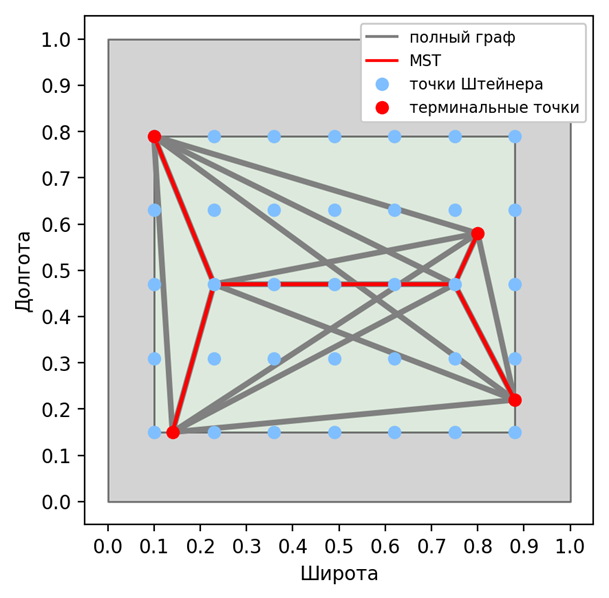
\includegraphics[width=0.7\textwidth]{images/4_2.png}
	\caption{Полный граф и MST}
\end{figure}
\vskip 4mm

Известно, что количество точек разветвления в итоговом графе не может превышать $n = |T| - 2$, где $|T|$ - количество терминальных точек. Будем добавлять точки разветвления итеративно. Мы строим полный граф между всеми терминальными точками и по очереди с каждой из точек разветвления, таким образом, что множество вершин полного графа состоит только из терминальных точек и точки разветвления. А весами рёбер этого графа является стоимость пути между этими вершинами в изначальном графе. После этого находим $MST$ и его вес. На нулевой итерации мы находим $MST$ без добавления точек разветвления. После того, как для каждой точки разветвления мы нашли $MST$, то нам нужно выбрать $MST$ минимального веса среди всех. Если добавление точки разветвления уменьшило вес $MST$ относительно прошлой итерации, то добавляем найденную точку разветвления в множество терминальных точек и повторяем цикл заново до тех пор, пока номер итерации не достигнет $n$ или добавление новой точки разветвления в граф не будет улучшать решение.\\
%\begin{algorithm}[H]
%	\SetAlgoLined
%	\KwData{$\mathbb{G}(\mathbb{V}, \mathbb{E})$ - взвешенный граф, $T \subseteq \mathbb{V}$  - набор терминальных точек }
%	\KwResult{$L_{res} = \{\{x_{j},y_{j}\}_{j=1}^{n_i}, i=\overline{1..s}\}$ - оптимальная сеть линейных объектов }
%	
%	$fork\_points$ := generate\_fork\_points($\mathbb{G}$, $T$)\\
%	$L_{res}$ := [...]\\
%	$m$ = $|T|$ - 2\\
%	\For{$\textbf{i = } 0 \textbf{ to } m-1$}
%	{
%		$all\_MSTs$ := [...]\\
%		$full\_graph$ := get\_full\_graph($\mathbb{G}$, $T$)\\
%		$MST$ := get\_MST($full\_graph$)\\
%		$min\_MST$ := MST\\		
%		$all\_MSTs.append(MST)$\\
%		
%		$T.append(node)$
%		
%	}
%	return $L_{res}$

%\caption{Алгоритм нахождения оптимальной сети}
%\end{algorithm}

\subsection*{\Large{Проведение измерений}}
Задача данного исследования найти зависимость между параметрами: временем работы программы и точностью получаемого решения. Для проведения этого исследования воспользуемся модельной картой в виде квадрата размером $[1.0 \times 1.0]$ градусов и построим вычислительную сетку с размером $d$ = 250 м. Параметры $n_x$  и $n_y$  будем варьировать в диапазоне $[3, \frac{width}{3d}]$ и $[3, \frac{height}{3d}]$, где $width$ и $height$ – ширина и высота ограничивающего прямоугольника в метрах. Будем строить дерево Штейнера для трех объектов. В качестве эталонного решения, возьмем решение, вычисленное аналитически (см. рис. 3).

\begin{figure}[H]
	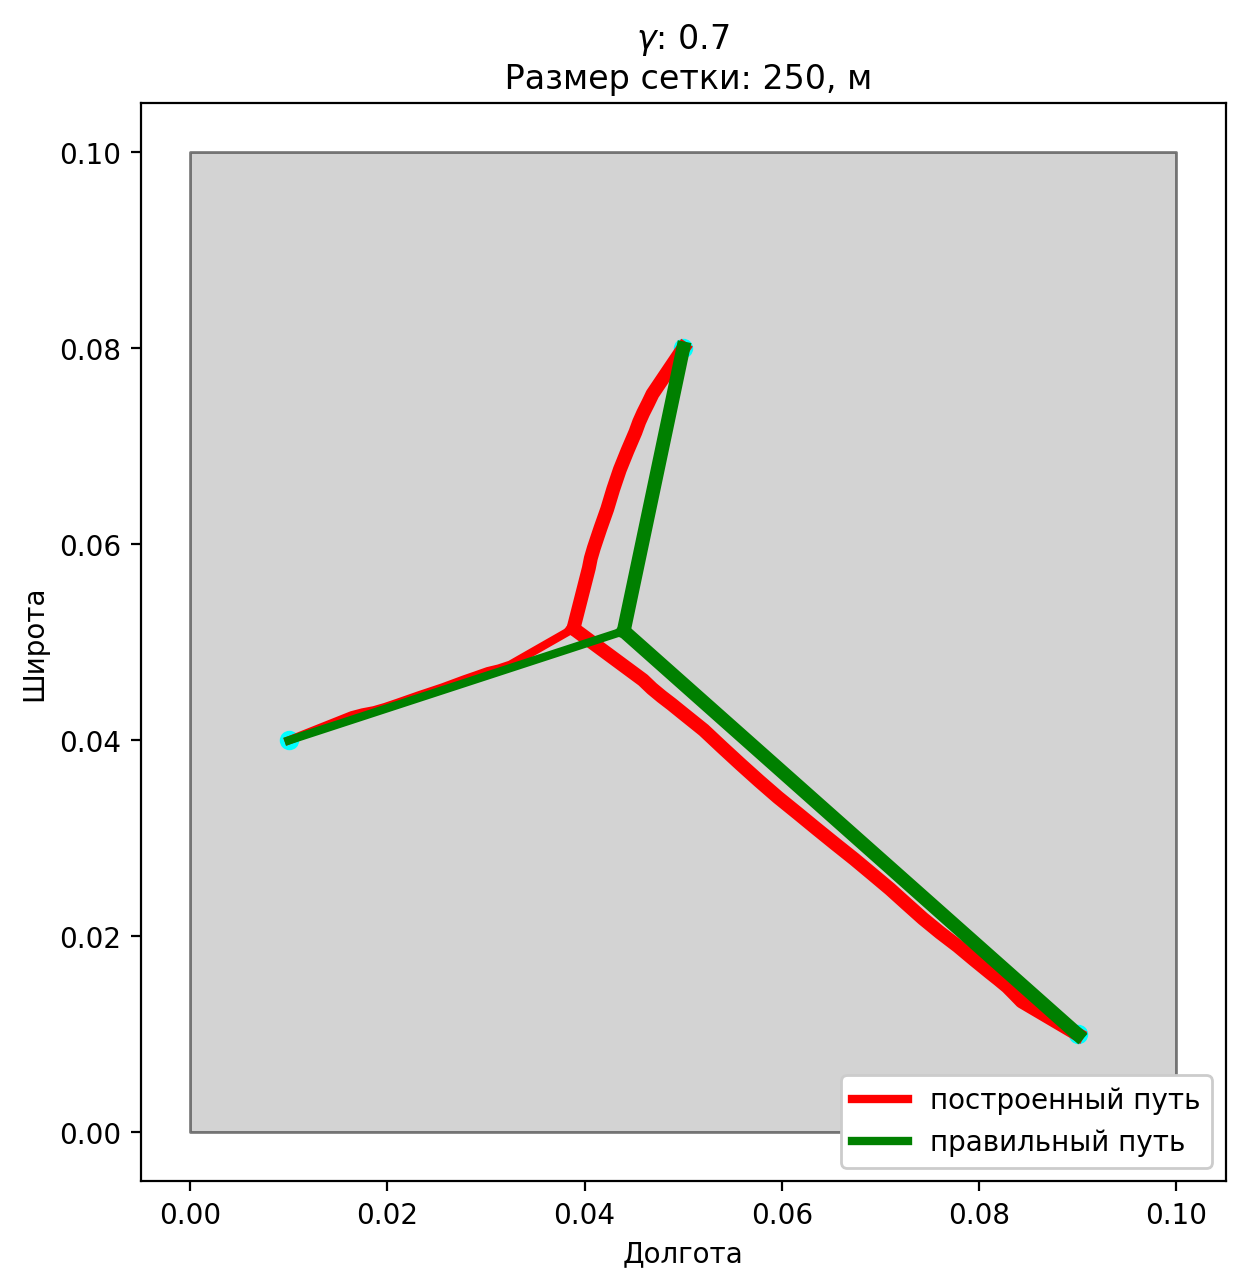
\includegraphics[width=0.7\textwidth]{images/4_3.png}
	\caption{Пример получившегося решения}
\end{figure}
\vskip 4mm


После выполнения вычислений была получена следующая таблица(см. табл. 1). Всего точек в графе 198025.

\begin{table}[H]
	\centering
	\caption{Результаты работы алгоритма}
	\begin{tabular}{|c|c|c|c|c|c|c|}
		\hline
		\textbf{Ошибка, \%} & \textbf{Время, сек} &	\textbf{$n_x$} &	\textbf{$n_y$} & \textbf{$n = n_x  \cdot n_y$} & \textbf{$\frac{time_{i}}{time_{i-1}}$} &	\textbf{$\frac{n_i}{n_{i-1}}$}   \\ \hline
		4.811675 &	3.009591 &	3 &	3 &	9 &	22.80485 &	15.88889 \\ \hline
		1.215535 &	68.63329 &	13 & 11 &	143 &	1.826607 &	3.356643 \\ \hline
		0.897341 &	125.366 &	24 & 20 &	480 &	1.884633 &	2.041667 \\ \hline
		1.060897 &	236.269 &	35 & 28 &	980 &	1.577195 &	1.736735 \\ \hline
		0.979378 &	372.6423 &	46 & 37 &	1702 &	1.426175 &	1.507051 \\ \hline
		1.016891 &	531.4531 &	57 & 45 &	2565 &	1.251421 &	1.410526 \\ \hline
		0.984747 &	665.0718 &	67 & 54 &	3618 &	1.331518 &	1.33665 \\ \hline
		0.938657 &	885.5548 &	78 & 62 &	4836 &	1.218663 &	1.306658 \\ \hline
		0.854584 &	1079.193 &	89 & 71 &	6319 &	1.17833 &	1.250198 \\ \hline
		0.924218 &	1271.646 &	100 & 79 &	7900 &	1.113036 &	1.236456 \\ \hline
		0.912585 &	1415.387 &	111	& 88 &	9768 &	None &	None \\ \hline
	\end{tabular}
\end{table}
\vspace{4mm}

Исходя из данных в этой таблице видно, что на плоскости качественные результаты можно получать при количестве точек разветвления в размере около 0.5-1\% от общего числа точек в ограничивающем прямоугольнике. Также можно заметить, что время работы программы практически линейно зависит от количества точек разветвления.










